\documentclass[10pt,twocolumn,letterpaper]{article}

\usepackage{cvpr}
\usepackage{times}
\usepackage{epsfig}
\usepackage{graphicx}
\usepackage{amsmath}
\usepackage{amssymb}

\usepackage{url}
\usepackage[T1]{fontenc}

% Include other packages here, before hyperref.

% If you comment hyperref and then uncomment it, you should delete
% egpaper.aux before re-running latex.  (Or just hit 'q' on the first latex
% run, let it finish, and you should be clear).
%\usepackage[pagebackref=true,breaklinks=true,letterpaper=true,colorlinks,bookmarks=false]{hyperref}

\cvprfinalcopy % *** Uncomment this line for the final submission

\def\cvprPaperID{****} % *** Enter the CVPR Paper ID here
\def\httilde{\mbox{\tt\raisebox{-.5ex}{\symbol{126}}}}

% Pages are numbered in submission mode, and unnumbered in camera-ready
\ifcvprfinal\pagestyle{empty}\fi
\begin{document}

%%%%%%%%% TITLE
\title{Lambda Architecture for Twitter real-time sentiment analysis}

\author{Lorenzo Agnolucci\\
E-mail address\\
{\tt\small lorenzo.agnolucci@stud.unifi.it}
% For a paper whose authors are all at the same institution,
% omit the following lines up until the closing ``}''.
% Additional authors and addresses can be added with ``\and'',
% just like the second author.
% To save space, use either the email address or home page, not both
}

\maketitle
\thispagestyle{empty}

%%%%%%%%% ABSTRACT
\begin{abstract}
With the increasing importance of social networks and Big Data in general in the modern society it is necessary to find some ways to analyze such a large amount of data. The Lambda Architecture was developed specifically to resolve this problem in an efficient and reliable way.

The aim of this work is to present a Lambda Architecture to perform a sentiment analysis on Twitter data in real-time using some of the frameworks of the Apache suite: Hadoop, HBase and Storm.
\end{abstract}

%%%%%%%%% BODY TEXT
\noindent\large\textbf{Future Distribution Permission}\\
\indent The author(s) of this report give permission for this document to be distributed to Unifi-affiliated students taking future courses.

\section{Introduction}
The advent of Big Data has brought a change in data processing over recent years. Big Data differs from traditional data processing through its use of parallelism: only by using multiple computing resources it is possible to process terabytes of data. The \textbf{Lambda Architecture} is a particular approach popularized by Nathan Marz that combines the large-scale batch-processing strengths of MapReduce with the real-time responsiveness of stream processing to allow to create scalable, responsive, and fault-tolerant solutions to Big Data problems \cite{butcher2014seven}. A Lambda Architecture is composed by 3 layers:
\begin{itemize}
\item \emph{batch layer}: it computes arbitrary functions on an immutable, constantly growing master database. It uses batch-oriented technologies like MapReduce to precompute batch views from historical data and this is effective but latency is high
\item \emph{serving layer}: it is a specialized distributed database that supports batch updates and random reads but does not need to support random writes
\item \emph{speed layer}: it only looks at recent data and uses low-latency techniques like stream processing to update the real-time views as it receives new data instead of recomputing the views from scratch. It compensates for the high latency of the batch layer
\end{itemize}
Real-time views contain only information derived from the data that arrived since the batch views were last generated and are discarded when the data they were built from is processed by the batch layer. The batch and real-time views are combined to create query results \cite{marz2015big}.

Sentiment analysis is a type of data mining that measures the inclination of people's opinions on a particular topic, product, person or brand through natural language processing (NLP), computational linguistics and text analysis.

For these reasons it is useful and appropriate to perform a sentiment analysis about certain keywords on Twitter data  using a Lambda Architecture.

%-------------------------------------------------------------------------
%-------------------------------------------------------------------------

\section{Proposed approach}

\begin{figure*}[t!]
\centering
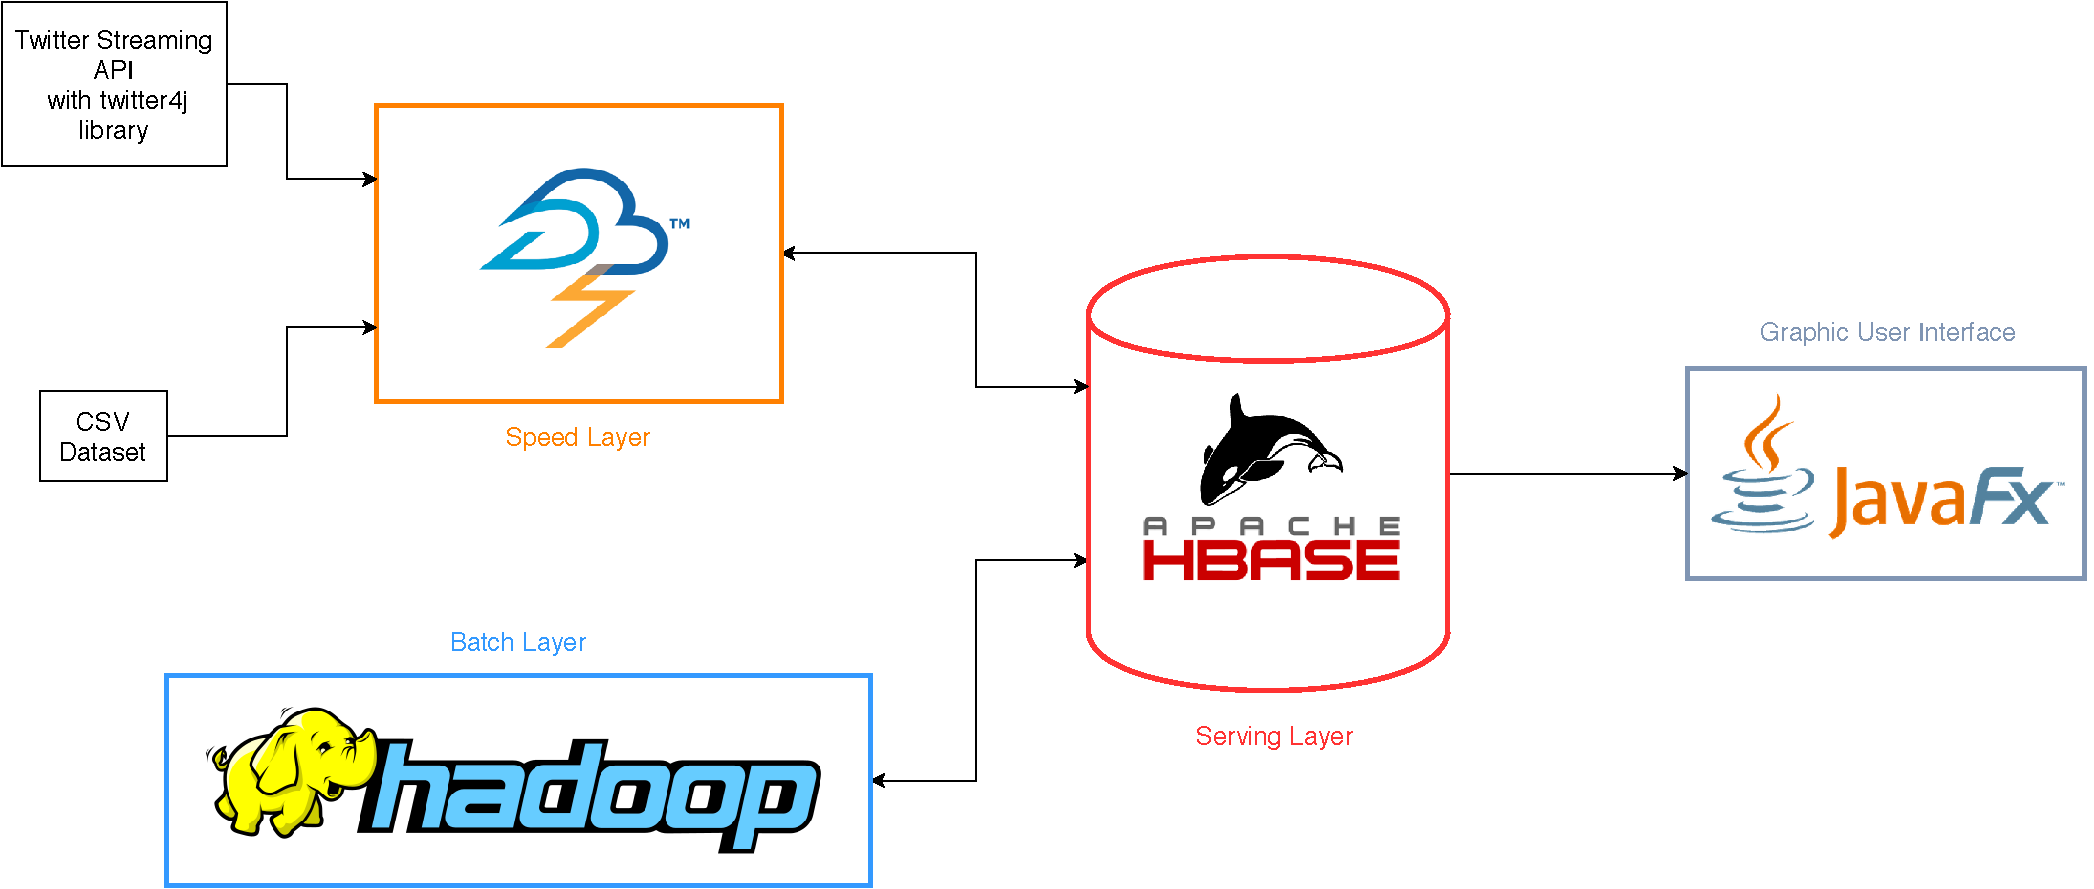
\includegraphics[width=0.99\linewidth]{img/lambda_architecture_diagram}
\vspace{0.5cm}
\caption{Diagram of the Lambda Architecture structure}
\label{fig:lambda_architecture_diagram}
\end{figure*}

The main goal of this work was not a perfect sentiment classification of tweets but rather the implementation of a Lambda Architecture capable of efficiently providing sentiment analysis statistics of tweets in real time. The project has been developed exclusively with Java, and \emph{Apache Storm} \cite{Storm}, \emph{Hadoop} \cite{Hadoop} and \emph{HBase} \cite{HBase} have been executed in a pseudo-distributed mode on a local cluster.

The speed layer represents the core of this work and it is started first. It takes as arguments the keywords on which the sentiment analysis will be performed by the whole architecture and creates the tables of the speed layer. Then the batch layer and the GUI are started so that the Lambda Architecture is complete.

To increase the number of tweets handled by the architecture (or in other words to avoid having to run the architecture for a long time) it is pretended that some tweets belonging to a dataset \cite{guyzGithubDataset} are taken from the real-time stream. Consistently some of the keywords taken as arguments by the speed layer match the keywords of the dataset (\eg $\#Apple$ and $\#Google$).

The structure of the proposed Lambda Architecture is shown in \emph{figure \ref{fig:lambda_architecture_diagram}}.

%-------------------------------------------------------------------------

\subsection{Sentiment classifier}
A sentiment classifier model has been trained using the \emph{LingPipe} library \cite{LingPipe} with a dataset \cite{go2009twitter} composed by 1.6 million tweets and with only \textbf{2 categories}: positive and negative. Then the trained model has been stored locally so that the batch and the speed layer could use it to classify other tweets. The model has also been evaluated with another dataset \cite{guyzGithubDataset} and despite the fact that the classification was not the main focus of this work it still achieved a decent 0.71 accuracy.

%-------------------------------------------------------------------------

\subsection{Serving Layer}
The serving layer uses \emph{Apache HBase}. The tables are created by the speed layer at the beginning of the execution. There are \textbf{4 tables}:
\begin{itemize}
\item \emph{tweet master database}: it represents the master database of the Lambda Architecture. Each row contains the text, the keywords and the ID of each tweet
\item \emph{tweet real-time database}: it contains only the information regarding the tweets that arrived since the batch view was last generated. Each row contains the keywords and the sentiment associated to a certain tweet and, as every other thing that is stored in \emph{HBase}, the timestamp in which the row was inserted in the database. In this case the timestamp is particularly useful because it is used to discard the rows corresponding to tweets already processed by the batch layer
\item \emph{batch view}: it is the result of the computation of the batch layer. It contains a row for each keyword and the number of positive and negative sentiments associated to it
\item \emph{synchronization table}: it is composed by only 2 rows that represent respectively the timestamps of the start and the end of the batch processing. These timestamps are used to synchronize the batch and the speed layer
\end{itemize}

%-------------------------------------------------------------------------

\subsection{Batch Layer}
The batch layer is represented by \emph{Apache Hadoop}, that runs in an infinite loop and computes a \textbf{MapReduce} job on \emph{tweet master database}, and then it writes its results from scratch in \emph{batch view}. It also writes the timestamps of the beginning and of the end of the execution in \emph{synchronization table}. 

The Mapper reads the text and the keywords of each tweet from \emph{tweet master database} and then classifies the text using the already trained sentiment classifier model. Then for each keyword contained in the text of the tweet it outputs a tuple structured as \emph{$<Keyword, Sentiment>$}. The Reducer takes a tuple in input and it increments the value of the column of the sentiment corresponding to the sentiment field of the tuple of the row associated to the keyword field of \emph{batch view}.

%-------------------------------------------------------------------------

\subsection{Speed Layer}

\begin{figure*}[t!]
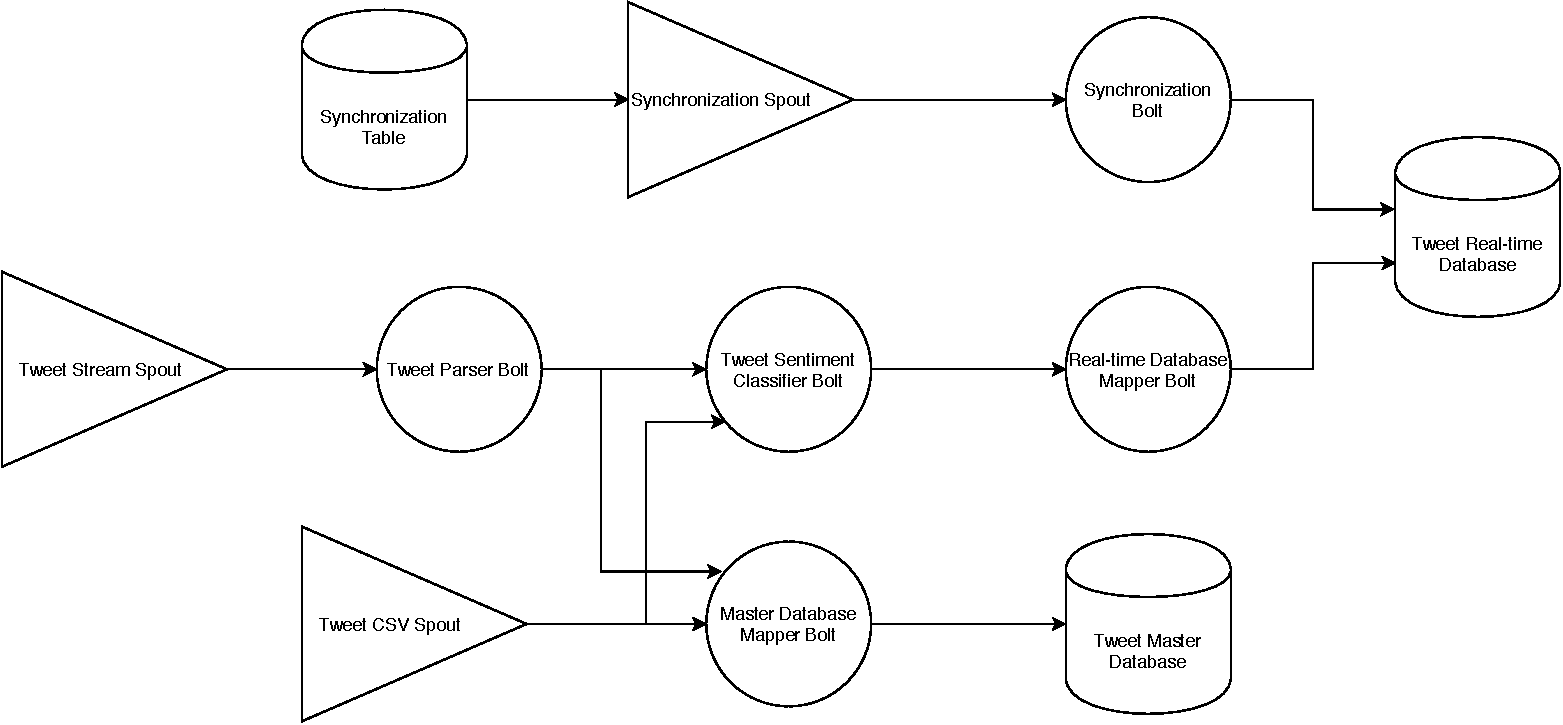
\includegraphics[width=0.95\linewidth]{img/storm_topology_diagram}
\vspace{0.5cm}
\caption{Diagram of the Storm topology}
\label{fig:storm_topology_diagram}
\end{figure*}

The core of the speed layer is \emph{Apache Storm}. The program takes the keywords as arguments and creates all the tables of the serving layer at the beginning of the execution (if they do not already exist).

To discard the data already processed by the batch layer from the real-time view it was necessary to implement \emph{synchronization spout} and \emph{synchronization bolt}, combined with \emph{synchronization table}. In this way when the batch layer terminates its execution the rows inserted before the start of the batch computation are no longer part of the real-time view. At the same time the rows inserted during the batch computation are not discarded and still are a part of the real-time view. The \textbf{Storm topology} (shown in \emph{figure \ref{fig:storm_topology_diagram}}) is composed by:
\begin{itemize}
\item \emph{tweet stream spout}: it uses the \emph{twitter4j} library and the Twitter Streaming API to get a real-time stream of tweets. It filters the tweets to retrieve only the ones that contain at least one of the keywords and that are written in English
\item \emph{tweet parser bolt}: it takes a tweet object in input and parse it to output a tuple containing the ID, the text and the keywords of the tweet
\item \emph{tweet CSV spout}: this spout would not exist in a real-world application but in this work it is used to increment the number of tweets computed by the Lambda Architecture. For each tweet of the dataset \cite{guyzGithubDataset} it outputs a tuple with the same structure used by \emph{tweet parser bolt}
\item \emph{master database mapper bolt}: it inserts a row in \emph{tweet master database} for each parsed tweet
\item \emph{tweet sentiment classifier bolt}: it uses the already trained sentiment classifier model to classify the text of the tweet. Then, for each keyword contained in the text it outputs a tuple containing the keyword and the infered sentiment
\item \emph{real-time database mapper bolt}: for each tuple outputted by \emph{twitter sentiment classifier bolt} it inserts a row in \emph{tweet real-time database}
\item \emph{synchronization spout}: it checks the two rows of the \emph{synchronization table} and when both the start and the end timestamps are modified it outputs a tuple containing the start timestamp
\item \emph{synchronization bolt}: it takes the start timestamp outputted by \emph{synchronization spout} and it deletes the rows of \emph{tweet real-time database} with a preceding timestamp
\end{itemize}

%-------------------------------------------------------------------------

\subsection{Data visualization}
To visualize the data and to better show how the different parts of the architecture work together a simple \textbf{Graphic User Interface} was developed with \emph{Java FX}. It is composed by two tables, representing respectively the content of the real-time view and the batch view, and a bar chart, which combines the data of the two views. The data of the batch view is retrieved straightforwardly from the \emph{batch view} table, as each of its rows represents the number of positive and negative sentiments associated to a specific keyword. On the contrary a more elaborated process is needed to get the real-time view: indeed it is necessary to aggregate the rows of the \emph{real-time database} with the same keyword and sentiment and count them. The content of both the views and the chart is refreshed every second to show the most recent results. \emph{Figure \ref{fig:GUI_screenshot}} shows a screenshot of the GUI.

\begin{figure}[h!]
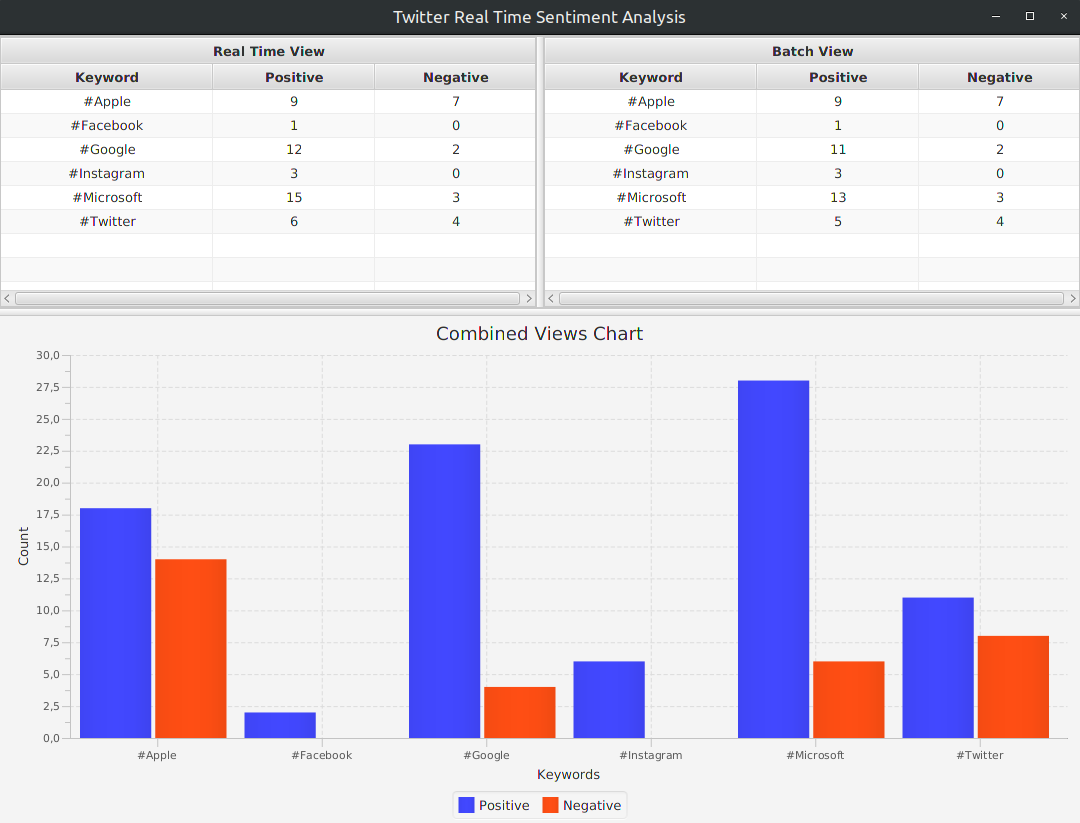
\includegraphics[width=0.98\linewidth]{img/GUI.png}
\vspace{0.25cm}
\caption{Screenshot of the GUI}
\label{fig:GUI_screenshot}
\end{figure}

%-------------------------------------------------------------------------
%-------------------------------------------------------------------------

\section{Conclusions and future work}
In the present work it has been shown an implementation of a Lambda Architecture capable of getting sentiment analysis statistics of real-time tweets. The GUI that was developed lets to understand simply and to visualize how the different parts of a Lambda Architecture work together in order to allow to handle a large amount of data efficiently and correctly.

As future developments a "neutral" category could be added to the sentiment classifier to better handle the tweets that not necessarily express an opinion on the keyword. Also, the architecture could be deployed to an Amazon Web Services cluster to exploit the fully distributed mode of Storm and Hadoop.

%-------------------------------------------------------------------------
%-------------------------------------------------------------------------

{\small
\bibliographystyle{ieee}
\bibliography{egbib}
}

\end{document}